% Use only LaTeX2e, calling the article.cls class and 12-point type.

\documentclass[12pt]{article}

% Users of the {thebibliography} environment or BibTeX should use the
% scicite.sty package, downloadable from *Science* at
% www.sciencemag.org/about/authors/prep/TeX_help/ .
% This package should properly format in-text
% reference calls and reference-list numbers.

%\usepackage{scicite}
\usepackage[numbers, square, sort, compress]{natbib}

% Use times if you have the font installed; otherwise, comment out the
% following line.

\usepackage{times}
\usepackage{hyperref}
\usepackage{graphicx}
\usepackage{amsmath}
\usepackage[left]{lineno}
\linenumbers
% The preamble here sets up a lot of new/revised commands and
% environments.  It's annoying, but please do *not* try to strip these
% out into a separate .sty file (which could lead to the loss of some
% information when we convert the file to other formats).  Instead, keep
% them in the preamble of your main LaTeX source file.


% The following parameters seem to provide a reasonable page setup.

\topmargin 0.0cm
\oddsidemargin 0.2cm
\textwidth 16cm 
\textheight 21cm
\footskip 1.0cm



% If your reference list includes text notes as well as references,
% include the following line; otherwise, comment it out.

\renewcommand\refname{References and Notes}

% The following lines set up an environment for the last note in the
% reference list, which commonly includes acknowledgments of funding,
% help, etc.  It's intended for users of BibTeX or the {thebibliography}
% environment.  Users who are hand-coding their references at the end
% using a list environment such as {enumerate} can simply add another
% item at the end, and it will be numbered automatically.

\newcounter{lastnote}
\newenvironment{scilastnote}{%
\setcounter{lastnote}{\value{enumiv}}%
\addtocounter{lastnote}{+1}%
\begin{list}
{\arabic{lastnote}.}
{\setlength{\leftmargin}{.22in}}
{\setlength{\labelsep}{.5em}}}
{\end{list}}


% Include your paper's title here

\title{Towards human Super EEG} 


% Place the author information here.  Please hand-code the contact
% information and notecalls; do *not* use \footnote commands.  Let the
% author contact information appear immediately below the author names
% as shown.  We would also prefer that you don't change the type-size
% settings shown here.

\author
{Lucy L. W. Owen$^{1}$, Andrew C. Heusser$^{1, 2}$, and Jeremy R. Manning$^{1\ast}$\\\\
$^{1}$Department of Psychological and Brain Sciences, Dartmouth College,\\
Hanover, NH 03755, USA\\
$^{2}$Akili Interactive,\\
Boston, MA 02110, USA}

% Include the date command, but leave its argument blank.

\date{}



%%%%%%%%%%%%%%%%% END OF PREAMBLE %%%%%%%%%%%%%%%%


\begin{document} 

% Double-space the manuscript.

\baselineskip24pt

% Make the title.

\maketitle 

\begin{abstract}
A growing body of literature over the past several decades reports that the dynamic correlational structure of functional neuroimaging data may be used to predict which moment of movie or story an individual is experiencing, identify which person's brain a recording came from, and identify the task a person is performing.  However, our structural (anatomical) connectome is roughly static for the duration of typical neuroimaging experiments.  How might these notions of dynamic functional connectomes versus static structural connectomes be reconciled?  We use two human electrocorticographic (ECoG) datasets to ask: to what extent can we use a static connectome model (trained using within versus across subject data, and within versus across task data) to explain dynamic full-brain activity patterns?  Given a fixed connectome model, and given recordings from a subset of brain locations, we test how reliably can one infer activity patterns throughout the rest of the brain.  Our model-based approach, termed \textit{SuperEEG}\footnote{The term ``Super EEG'' was
coined by Robert J. Sawyer in his popular science fiction novel
\textit{The Terminal Experiment}~\cite{Sawy95}}, is in itself useful for inferring full-brain activity patterns (at millimeter-scale spatial resolutions and millisecond-scale temporal resolutions) from ECoG recordings from a limited set of brain locations.  For both datasets, we found that full-brain activity patterns can be best explained using connectomes from \textit{other} people who performed a shared task.\\

\small{\textbf{Keywords: Electrocorticography (ECoG), intracranial electroencephalography (iEEG),
local field potential (LFP), epilepsy, maximum likelihood estimation, Gaussian process regression}}
\end{abstract}

Are our brain's networks static or dynamic?  And to what extent are the network properties of our brains stable across people and tasks?  One body of work suggests that our brain's \textit{functional} networks are dynamic~\citep[e.g., ][]{MannEtal18}, person-specific~\citep[e.g., ][]{FinnEtal15}, and task-specific~\citep[e.g., ][]{Turk13}.  In contrast, although the gross anatomical structure of our brains changes meaningfully over the course of years as our brains develop, on the timescales of typical neuroimaging experiments (i.e., hours to days) our anatomical networks are largely stable~\citep[e.g., ][]{CaseEtal00}.  Further, many aspects of brain anatomy, including white matter structure, is largely preserved across people~\citep[e.g., ][]{TalaTour88, JahaEtal13, MoriEtal08}  There are several possible means of reconciling this apparent contradiction between dynamic person- and task-specific functional networks versus stable anatomical networks.  For example, relatively small magnitude anatomical differences across people may be reflected in reliable functional connectivity differences.  Along these lines, one recent study found that diffusion tensor imaging (DTI) structural data is similar across people, but may be used to predict person-specific resting state functional connectivity data~\citep{BeckEtal18}.  Another (potentially complementary) possibility is that our functional networks are constrained by anatomy, but nevertheless exhibit rapid task-dependent changes~\citep[e.g., ][]{SporBetz16}.

Here we take a model-based approach to studying whether high spatiotemporal resolution activity patterns throughout the human brain may be explained by a static connectome model that is shared across people and tasks.  Specifically, we trained a model to take in recordings from a subset of brain locations, and then predict activity patterns during the same interval, but at \textit{other} locations that were held out from the model.  Our model, based
on Gaussian process regression, relies on three assumptions (each of which we test).  First, we assume that functional correlations are stable over time and across tasks.  Second, we assume that some of the correlational structure of people's brain activity is similar across individuals.  Third, we resolve
ambiguities in the data by assuming that neural activity from
nearby sources will tend to be similar, all else being equal.  After fitting the model to an ECoG dataset, one
can then ask (for a held-out individual's brain): given what we
know about the correlational structure of \textit{other} people's brains,
and given the recordings we made from electrodes implanted in this
person's brain, how would those recordings most likely have looked
at \textit{other} locations throughout this person's brain?  We named our general approach \textit{SuperEEG} because the trained model provides a means of inferring full-brain activity patterns at high spatiotemporal resolutions, using ECoG recordings taken from a limited set of brain locations.  

We tested the SuperEEG approach using two large ECoG datasets. Dataset 1 comprises multi-hour recordings from 6876 electrodes taken across several recording sessions as 88 neurosurgical patients studied random word lists periodically throughout their day~\cite{SedeEtal03, SedeEtal07a,
  SedeEtal07b, MannEtal11, MannEtal12}.  Dataset 2 comprises recordings from XXX electrodes taken as XXX patients performed a series of two memory tasks~\citep{EzzyEtal17, HoraEtal17, KragEtal17, KuceEtal17, LinEtal17, SoloEtal18, WeidEtal18, EzzyEtal18, KuceEtal18}.  In both datasets, 
  we compared the predictions made using models trained across people to predictions made using within-person data.  We found that models that incorporate data from other patients yield far more reliable predictions about an individual patient's brain activity patterns than models trained solely on that individual's data.  This indicates that at least some functional correlations are common across people.  We also used Dataset 2 to compare predictions made using data from within task, across task, or combining within and across task data.  We found that all three approaches yielded reliable predictions, but the within task predictions were the most accurate.  This indicates that some aspects of our functional connectomes are common across tasks, whereas other aspects are task-specific.  Finally, all of the models we trained (within and across patients and tasks) assumed a static connectome and yielded above-chance accuracy.  This indicates that despite moment-by-moment fluctuations in the functional connectome, at least some aspects of our connectome appear to be stable over the course of several hours.

\textbf{JRM STOPPED HERE}
\section*{Approach}
The SuperEEG approach to inferring high temporal resolution full-brain activity patterns is outlined and summarized in
Figure~\ref{fig:methods}. We describe (in this section) and evaluate
(in \textit{Results}) our approach using a two large previously collected
dataset comprising multi-session intracranial recordings.  The first dataset was taken from
6876 electrodes implanted in the brains of 88 epilepsy
patients~\cite{SedeEtal03, SedeEtal07a, SedeEtal07b, MannEtal11,
  MannEtal12}.  We first applied a fourth order Butterworth notch filter to remove
60 Hz ($\pm$ .5 Hz) line noise.  We then excluded any electrodes that
showed putative epileptiform activity.  Specifically, we excluded from
further analysis any electrode that exhibited an average kurtosis of
10 or greater across all of that patient's recording sessions.  We
also excluded any patients with fewer than 2 electrodes that passed
this criteria, as the Super EEG algorithm requires measuring
correlations between 2 or more electrodes from each patient.
Altogether this yielded clean recordings from 4168 electrodes
implanted throughout the brains of 67 patients (Fig.~\ref{fig:methods}A). For the purposes of comparing task-specific contributions to reconstruction accuracy, we limited our analyses in the second dataset to patients that participated in two free recall experiments.  Applying the same kurtosis thresholding yielded clean recordings from 24 patients and 2975 electrodes for the second dataset. Each individual patient contributes
electrodes from a limited set of brain locations, which we localized
in a common space (MNI152); an example patient's 54 electrodes that
passed the predefined kurtosis test are highlighted in black and red.


The recording from a given electrode is maximally informative about
the activity of the neural tissue immediately surrounding its
recording surface.  However, brain regions that are distant from the
recording surface of the electrode also contribute to the recording,
albeit (often) to a much lesser extent.  One mechanism underlying these
contributions is volume conduction.  The precise rate of falloff due
to volume conduction (i.e. how much a small volume of brain tissue at
location $x$ contributes to the recording from an electrode at
location $\eta$) depends on the size of the recording surface, the
electrode's impedance, and the conductance profile of the volume of
brain between $x$ and $\eta$.  As an approximation of this intuition,
we place a Gaussian radial basis function (RBF) at the location $\eta$
of each electrode's recording surface (Fig.~\ref{fig:methods}B).  We
use the values of the RBF at any brain location $x$ as a rough
estimate of how much structures around $x$ contributed to the
recording from location $\eta$:

\begin{align}
  \mathrm{rbf}(x|\eta,\lambda) & =
  \mathrm{exp}\left\{ -\frac{||x - \eta||^2}{\lambda} \right\},\label{eqn:rbf}
\end{align}
where the width variable $\lambda$ is a parameter of the algorithm
(which may in principle be set according to location-specific tissue
conductance profiles) that governs the level of spatial smoothing.  In
choosing $\lambda$ for the analyses presented here, we sought to
maximize spatial resolution (which implies a small value of $\lambda$)
while also maximizing the algorithm's ability to generalize to any
location throughout the brain, including those without dense electrode
coverage (which implies a large value of $\lambda$). Using our prior
work as a guide~\cite{MannEtal14b}, we set $\lambda = 20$, although
this could in theory be optimized, e.g. using cross validation.


\begin{figure}
  \centering
  \includegraphics[width=\textwidth]{figs/methods}
  \caption{\textbf{Methods overview.}  \textbf{A.  Electrode
      locations.}  Each dot reflects the location of a single
    electrode in dataset 1, colored according to 7 factor labels (see Panel D for details). One patient's electrode locations are
    highlighted in black and the to-be-reconstructed recording location
    is highlighted in red. \textbf{B. Radial basis function (RBF).}
    Each electrode contributed by the patient (black) weights on the
    full set of locations under consideration (all dots in Panel A,
    defined as $\bar{R}$ in the text).  The weights fall off with
    positional distance (in MNI space) according to an RBF.
    \textbf{C. Per-patient correlation matrices.}  After computing the
    pairwise correlations between the recordings from each patient's
    electrodes, we use RBF-weighted averages to estimate correlations
    between all locations in $\bar{R}$.  We obtain an estimated
    full-brain correlation matrix using each patient's
    data. \textbf{D.  Combined correlation matrix.}  We estimate a
    single full-brain correlation matrix by averaging 
    the patient-specific correlation matrices.  We sort the resulting correlation matrix based on 7 factor labels obtained from k-means clustering~\cite{YeoEtal11}). \textbf{E.
      Reconstructing activity throughout the brain.}  Given the observed
    activity from the patient's electrodes and the estimated
    correlation matrix (Panel D), we can compute a maximum likelihood
    estimate of the voltage trace at any location in $\bar{R}$.  An
    example reconstruction (at the red dot in Panel A) is shown in
    red, and the actual recording at that location is highlighted above in blue.}
  \label{fig:methods}
\end{figure}

A second mechanism whereby a given region $x$ can contribute to the
recording at $\eta$ is through anatomical connections between
structures near $x$ and $\eta$.  We use spatial correlations in the
data to estimate these anatomical connections.  Let $\bar{R}$ be the
set of locations at which we wish to estimate local field potentials,
and let $R_{s}$ be set of locations at which we observe local field
potentials from patient $s$ (excluding the electrodes that did not
pass the kurtosis test described above). In the analyses below we
define $\bar{R} = \cup_{s=1}^S R_s$.  We can calculate the expected
inter-electrode correlation matrix for patient $s$, where
$C_{s,k}(i,j)$ is the correlation between the time series of voltages
for electrodes $i$ and $j$ from subject $s$ during session $k$, using:

\begin{align}
  \bar{C}_{s} &=
  \mathrm{r}(\frac{1}{n}(\sum_{k=1}^{n}\mathrm{z}(C_{s,k}))),\label{eqn:inter_corr}~\mathrm{where}\\
\mathrm{z}(r) &= \frac{\log(1+r) - \log(1 - r)}{2}~\mathrm{is~the~Fisher}~z \mathrm{-transformation~and}\label{eqn:fishersz}\\
\mathrm{z}^{-1}(z) = \mathrm{r}(z) &= \frac{\exp(2z) - 1}{\exp(2z) + 1}\mathrm{~is~its~inverse}.\label{eqn:invfishersz}
\end{align}
Next, we use Equation~\ref{eqn:rbf} to construct a number of
to-be-estimated locations by number of patient electrode locations
weight matrix, $W$.  Specifically, $W$ approximates how informative the
recordings at each location in $R_s$ are in reconstructing activity at
each location in $\bar{R}$, where the contributions fall off with an RBF according to
the distances between the corresponding locations:

\begin{align}
W(i, j) = \mathrm{rbf}(i|j,\lambda)\label{eqn:weight_matrix}.
\end{align}

Given this weight matrix, $W$,
and the observed inter-electrode correlation matrix for patient $s$,
$\bar{C}_{s}$, we can estimate the correlation matrix for all locations in
$\bar{R}$ (Fig.~\ref{fig:methods}C) using:

\begin{align}
\hat{N}_{s}(x,y) & = { \sum_{i = 1}^{| R_{s}|}\sum_{j=1}^{i-1} W(x,i) \cdot W(y,j)\cdot \mathrm{z}(\bar{C}_{s}(i,j))}\label{eqn:correlation_matrix_num}\\
 \hat{D}_{s}(x,y) & = \sum_{i = 1}^{| R_{s}|}\sum_{j=1}^{i-1} W(x,i) \cdot W(y,j). \label{eqn:correlation_matrix_den}
\end{align}
Intuitively, we construct an estimated correlation matrix from each
individual patient's data (Fig.~\ref{fig:methods}C) using
Equations~\ref{eqn:correlation_matrix_num} \& \ref{eqn:correlation_matrix_den}, then we sum across these estimates for $S$ patients and divide (see Equations~\ref{eqn:correlation_matrix}) to obtain the expected correlation
matrix, $\hat{K}$ (Fig.~\ref{fig:methods}D):

\begin{align}
 \hat{K} = \mathrm{r} \left (  \frac{\sum  \hat{N}_{s}}{\sum \hat{D}_{s}}\right ).\label{eqn:correlation_matrix}
\end{align}
Now we can use the following intuition: given (i) the observed
responses from a limited set of locations in $R_{s}$ ($Y_{s}$) and
(ii) how each location's responses relate to all other responses
($\hat{K}$), we can estimate the LFP data from patient
$s$, for any arbitrary location in $\bar{R}$
(Fig.~\ref{fig:methods}E).

Let $\alpha$ be the set of indices of patient $s$'s electrode locations in
$\bar{R}$, and let $\beta$ be the set of indices of all other
locations in $\bar{R}$. In other words, $\beta$ reflects the locations
in $\bar{R}$ where we did not observe a recording for patient $s$
(these are the recording locations we will want to fill in using Super EEG).
We can sub-divide $\hat{K}$ as follows:

\begin{align}
\hat{K}_{\beta,\alpha} &= \hat{K}(\beta,\alpha),~\mathrm{and}\label{eqn:Kba}\\
\hat{K}_{\alpha,\alpha} &= \hat{K}(\alpha,\alpha)\label{eqn:Kaa}.
\end{align}
Here $\hat{K}_{\beta, \alpha}$ stores the correlations between the
``unknown'' activity at the locations in $\beta$ and the observed
activity at the locations in $\alpha$, and $\hat{K}_{\alpha, \alpha}$
stores the correlations between the observed recordings (at the
locations in $\alpha$). 

Let $Y_{s,k,\alpha}$ be the number-of-timepoints
($T$) by length($\alpha$) matrix of (observed) voltages from the electrodes in $\alpha$ during session $k$ from patient $s$. Then we can estimate the voltage from patient $s$'s $k^{th}$ session at the locations in $\beta$ using~\cite{Rasm06}:

\begin{align}
Y_{s,k,\beta} &= ((\hat{K}_{\beta,\alpha}\cdot\hat{K}_{\alpha,\alpha}^{-1})\cdot Y_{s,k,\alpha}^\mathrm{T})^\mathrm{T}.\label{eqn:reconstruction}
\end{align}
This equation is the foundation of the Super EEG algorithm.  Whereas
we observe the recordings only at the locations in $\alpha$,
Equation~\ref{eqn:reconstruction} allows us to estimate the recordings
at all locations in $\beta$, which we can define \textit{a priori} to
include any locations we wish, throughout the brain.  This yields estimates of
the time-varying voltages at \textit{every} location in $\bar{R}$.

We designed our approach to be agnostic to electrode impedances, as
electrodes that do not exist do not have impedances.  Therefore our
algorithm recovers voltages in standard deviation ($z$-scored) units
rather than attempting to recover absolute voltages. (This property
reflects the fact that $\hat{K}_{\beta, \alpha}$ and
$\hat{K}_{\alpha, \alpha}$ are correlation matrices rather than
covariance matrices.)  Also, note that
Equation~\ref{eqn:reconstruction} requires computing a $T$ by $T$
matrix, which can become computationally intractable when $T$ is very
large (e.g.\ for the patient highlighted in Fig.~\ref{fig:recon}, $T = 20458799$). However, we may approximate $Y_{s,k,\beta}$ in a piecewise
manner by filling in $Y_{s,k,\beta}$ in blocks of size $b$ samples
(using the corresponding samples from $Y_{s, k, \alpha}$).  In our
computations we set $b = 25000$.

The Super EEG algorithm described above and in
Figure~\ref{fig:methods} allows us to estimate (up to a constant
scaling factor) LFPs for each patient at all arbitrarily chosen
locations in the set $\bar{R}$, \textit{even if we did not record that
  patient's brain at all of those locations}.

\section*{Results}
To test the accuracy with which the Super EEG algorithm reconstructs activity throughout the brain, we held out each electrode from the full
dataset in turn and treated it as unobserved. We then asked: how
closely did each of the Super EEG-reconstructed LFPs match the
observed data?  We sought to evaluate both the overall reconstruction
accuracy as well as how reconstruction accuracy varied as a function
of implantation location.

We first examined raw LFP traces and their associated Super
EEG-derived reconstructions.  Figure~\ref{fig:recon}A displays the
LFP from the red electrode in Figure~\ref{fig:methods}A, and its
associated reconstruction, during a 5~s time window during one of the
patient's 6 recording sessions.  Figure~\ref{fig:recon}B displays a 2D
histogram of the observed versus reconstructed voltages for every
sample across 14.2 total hours of recordings from that patient (correlation:
$r = 0.91, p < 10\textsuperscript{-10}$).  Although the Super EEG
algorithm recovered the recordings from this electrode well, we sought to
quantify the algorithm's performance across the full dataset.

%sample trace & reconstruction, several frames of activity snapshot?
\begin{figure}
  \centering
  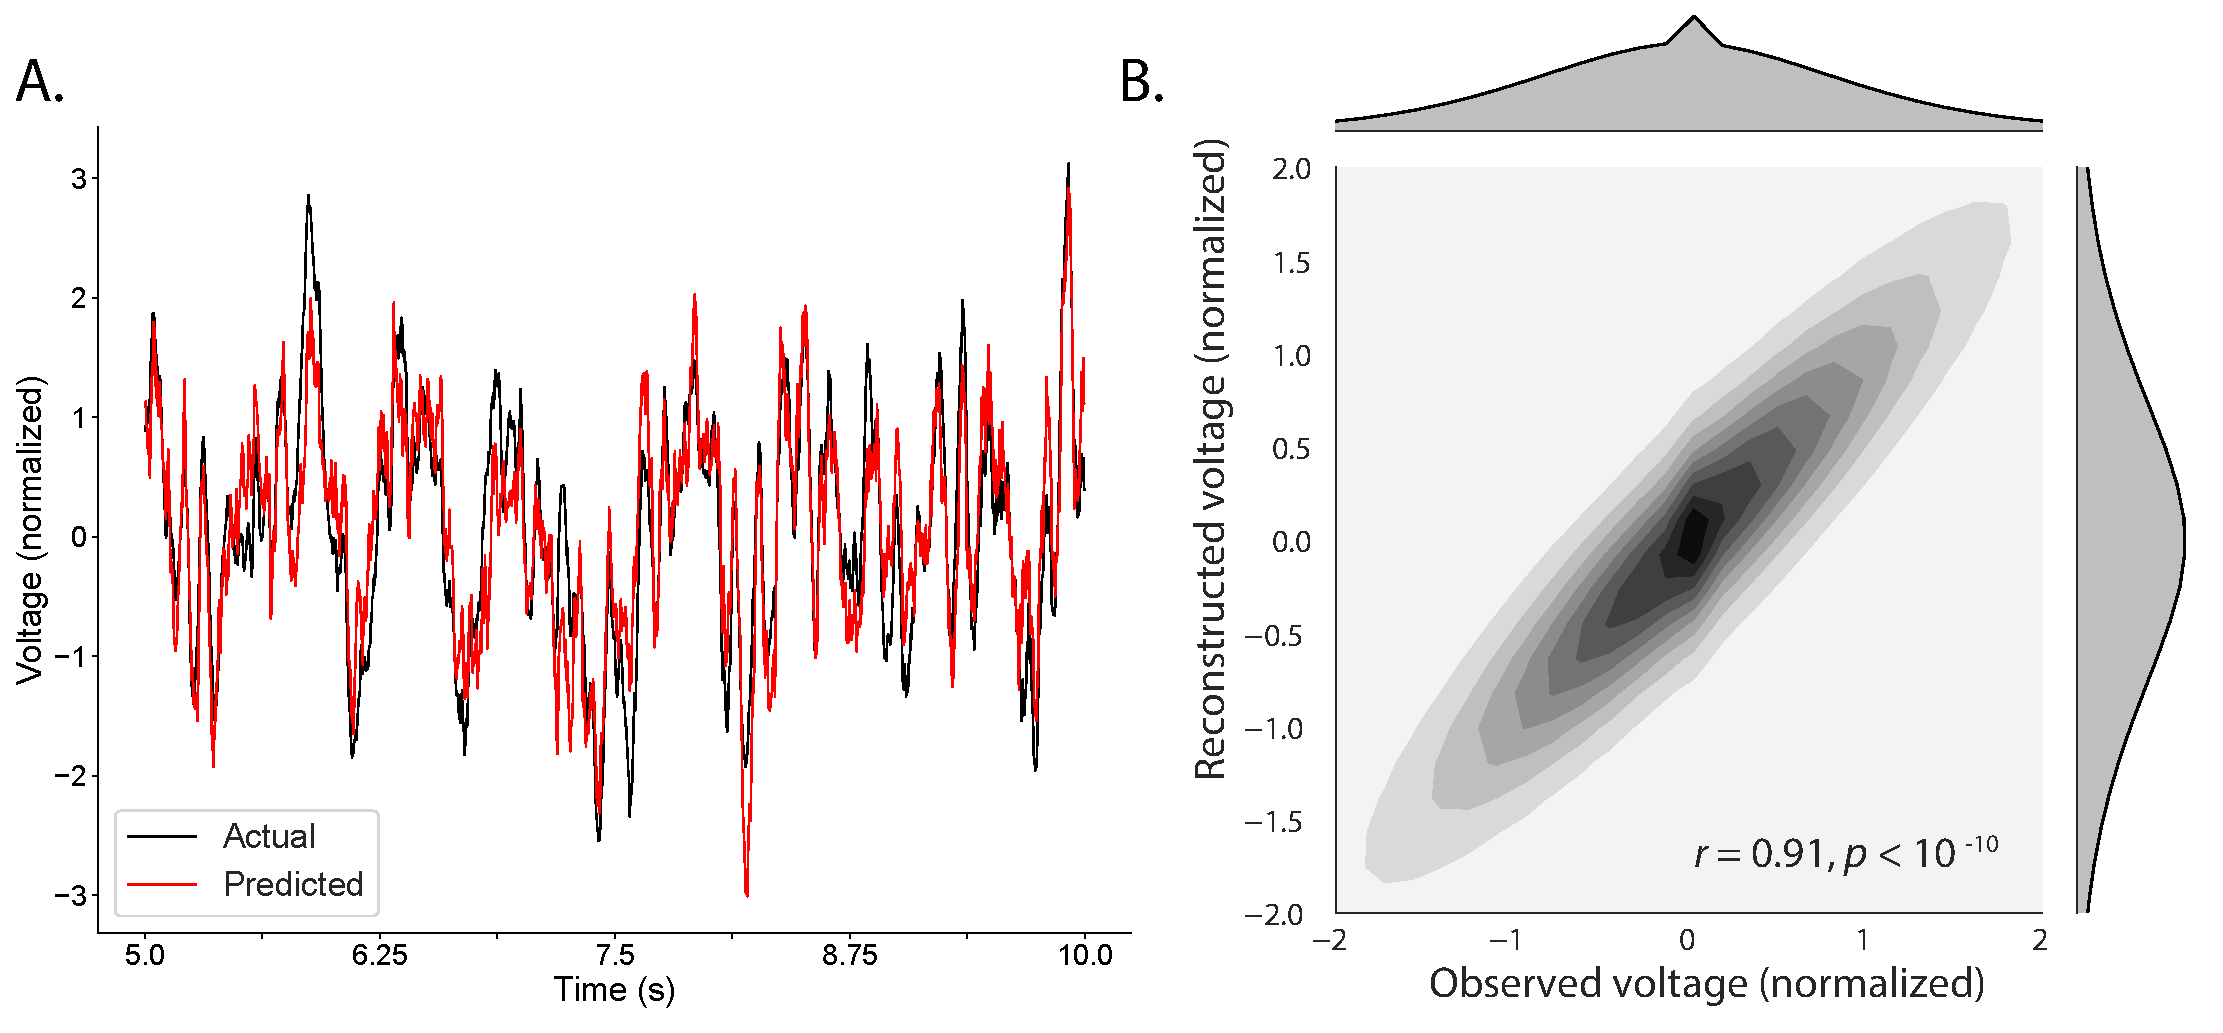
\includegraphics[width=\textwidth]{figs/recon}
  \caption{\textbf{Observed and reconstructed LFP from a single
      electrode.} \textbf{A. Example LFP.}  A 2~s recording from the blue
    electrode in Figure~\ref{fig:methods}A is displayed in red, and
    the reconstructed LFP during the same time window is shown in
   black.  All voltages are plotted in standard deviation units.
    \textbf{B. Observed versus reconstructed voltages over 14.2~hours.}
    The 2D histogram reflects the relation between distributions of
    observed versus reconstructed voltages from one patient, across the
    14.2 hours of recorded data collected in 6 recording sessions.  The
    correlation reported in the panel is between the observed and reconstructed
    voltages.}
  \label{fig:recon}
\end{figure}

Holding out each electrode from each patient in turn, we computed the
average correlation (across recording sessions) between the Super
EEG-reconstructed voltage traces and the observed voltage traces from
that electrode.  For each reconstruction, we estimated the full-brain
correlation matrix using every \textit{other} patient's data
(i.e. every patient except the one who contributed the
to-be-reconstructed electrode data).  In our analyses, we then
substituted the average correlation matrix computed after excluding
patient $s$'s data for $\hat{K}$ in Equations~\ref{eqn:Kba} and
\ref{eqn:Kaa}.  This step ensured that the data we were reconstructing
could not also be used to estimate the between-location correlations
that drove the reconstructions via Equation~\ref{eqn:reconstruction}
(otherwise the analysis would be circular).

We obtained a single correlation coefficient for each electrode
location in $\bar{R}$, reflecting how well the Super EEG algorithm was
able to recover the recording at that location by incorporating data across patients (Across shown in black, see Fig.~\ref{fig:corrmap}A). We also reconstructed activity for each electrode using a model trained on the remaining electrodes from only that patient, to account for reconstruction accuracy attributed to volume conductance alone (Within shown in gray, see Fig.~\ref{fig:corrmap}A). For the first dataset, we compared these two distributions of correlation coefficients (paired $t$-test
between $z$-transformed mean correlation coefficients by patient:
$t(66) = 9.64, p < 10\textsuperscript{-10}$).  We repeated this analysis on a similar dataset Fig.~\ref{fig:corrmap}C) with similar results (paired $t$-test
between $z$-transformed mean correlation coefficients by patient: $t(23) = 6.93, p < 10\textsuperscript{-5}$). This is an especially conservative
test, given that the Super EEG reconstructions exclude (from the
correlation matrix estimates) all data from the patient whose data is
being reconstructed.  Furthermore, we also replicated this finding for each independent experiment within dataset 2 (Fig. S3 (paired $t$-test
between $z$-transformed mean correlation coefficients by patient for experiment 1: $t(23) = 6.23, p < 10\textsuperscript{-5}$ and experiment 2: $t(23) = 6.62, p < 10\textsuperscript{-5}$).  That the Super EEG-derived correlations were reliably
stronger than these correlations obtained using a volume conductance null model is exciting
for two reasons.  First, it implies that distant electrodes provide
additional predictive power to the data reconstructions beyond the
information contained in nearby electrodes.  Second, it implies that
the spatial correlations driving the Super EEG algorithm are, to some
extent, shared across people.

%correlations by brain area, distribution of correlations
\begin{figure}
  \centering
  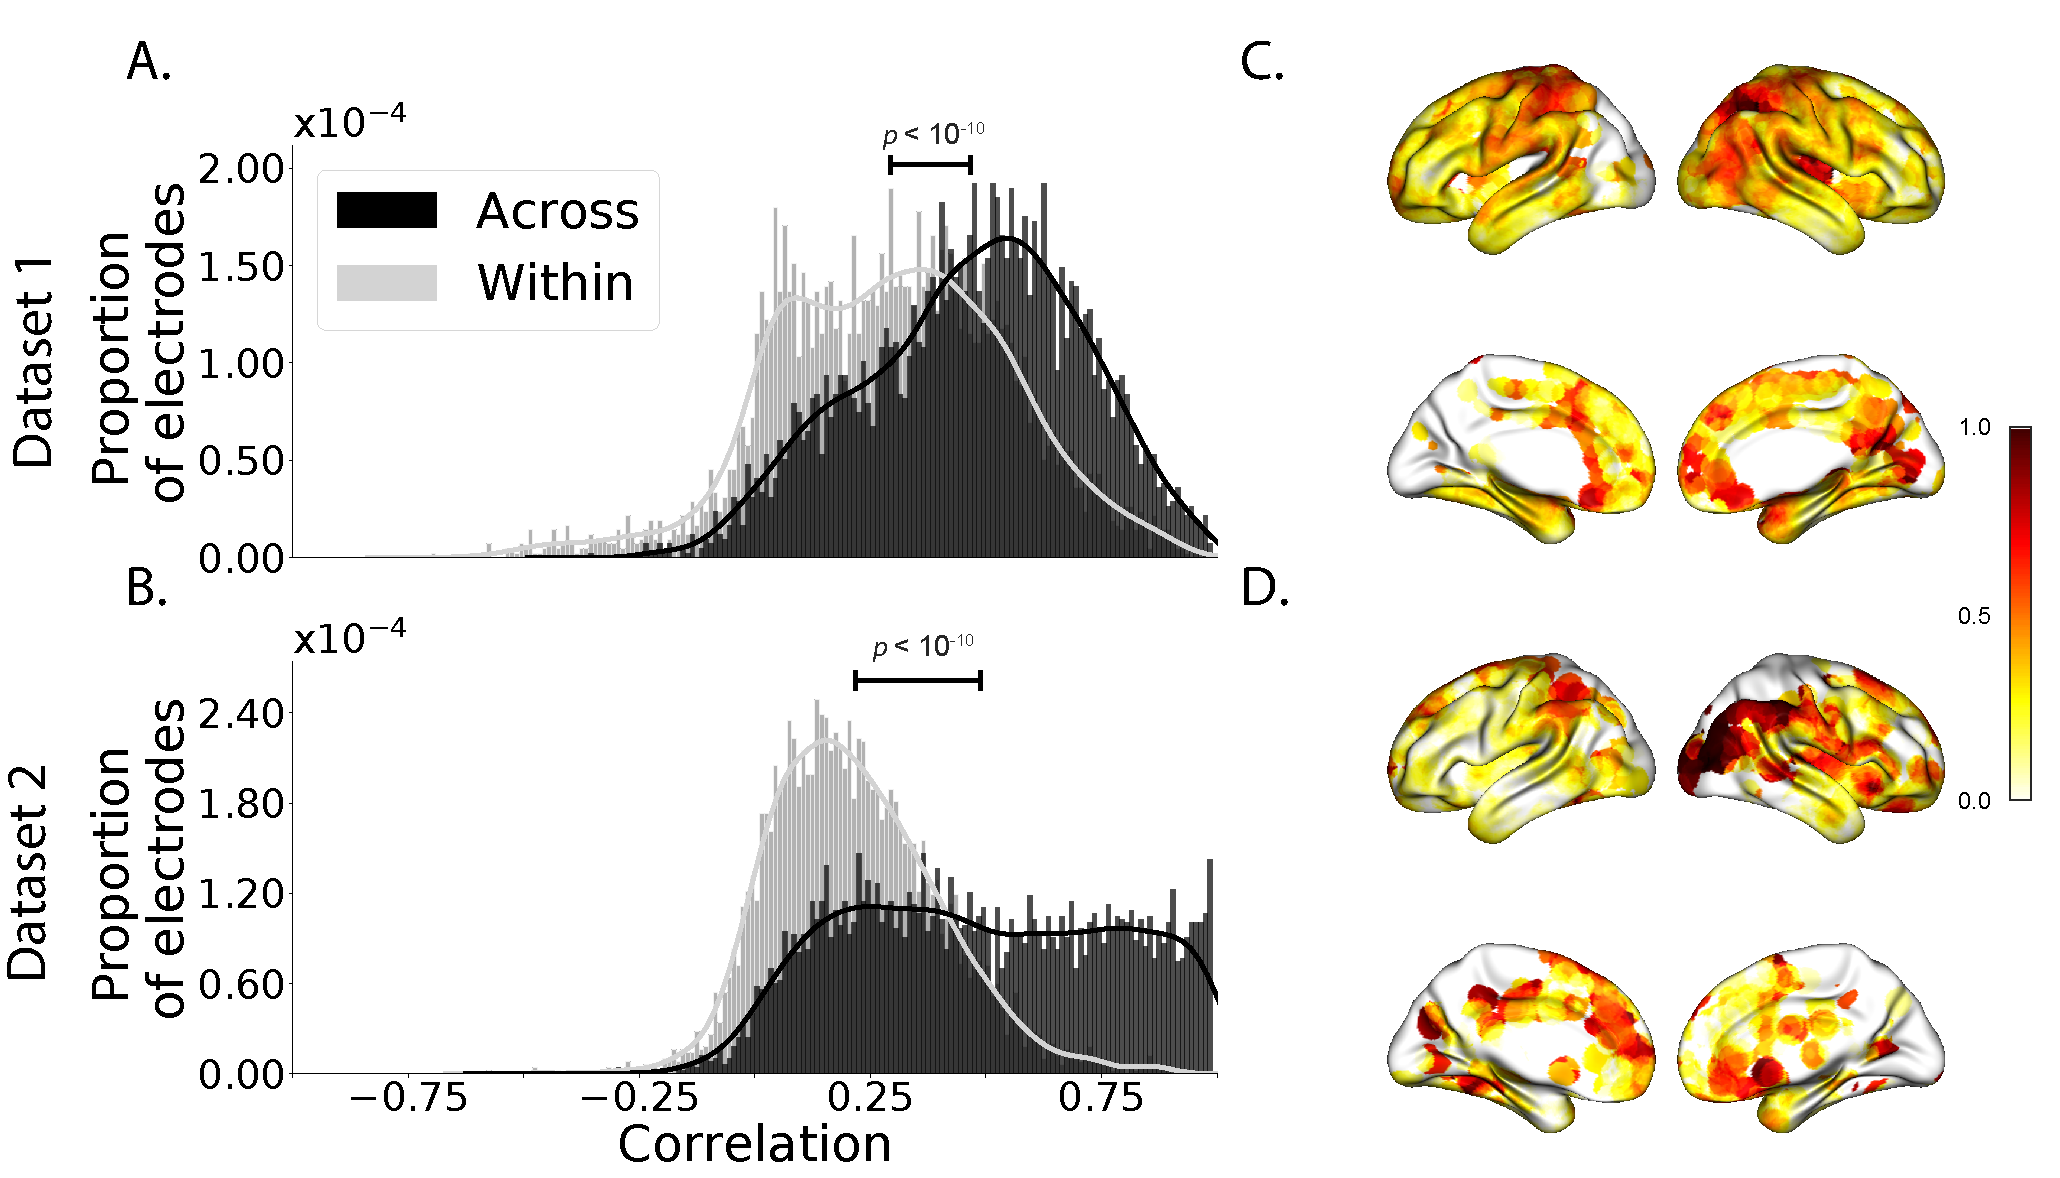
\includegraphics[width=\textwidth]{figs/corrmap}
  \caption{\textbf{Reconstruction quality.}  \textbf{A. \& C.  Distributions
      of correlation coefficients.}  Across all electrodes from all
    patients in the labeled dataset, the panel displays the distribution of correlations between the observed and reconstructed LFP data using models trained on data from all other patients (Across, in black) and all other electrodes from the same patient (Within, in gray). 
    \textbf{B. \& D. Correlation maps.}  The glass brain maps display the
    average correlation between the observed LFP data and the across-subjects model reconstructed data by location, for each labeled experiment.}
  \label{fig:corrmap}
\end{figure}

We were interested in the task specific contributions to the reconstruction accuracy.  Each patient in the the second dataset participated in two free recall experiments.  We ran similar analyses for both experiments and found that activity was best reconstructed when limiting the training data to within task, as opposed to across task or incorporating data from both tasks (Fig. S1 (mean reconstruction accuracy incorporating data within task: 0.55, across task: 0.37, all tasks: .50)). Although reconstruction accuracy in the across task analysis was still better than the volume conductance model alone (paired $t$-test
between $z$-transformed mean correlation coefficients by patient: $t(47) = 5.65, p < 10\textsuperscript{-5}$), these results suggests that having a common tasks for patients may yield better reconstruction accuracy.  

We also wondered whether reconstruction quality (measured as the
correlation between the observed and reconstructed data) varied with
the electrode locations (Fig.~\ref{fig:corrmap}B \& D). In general, reconstruction quality remained high throughout the brain. Although reconstruction accuracy appeared high in the medial temporal lobe, which is a common epileptic focus (and therefore a common target for electrode implantation), we observed a weak but statistically reliable negative correlation between reconstruction quality and electrode density (defined as the proportion of electrodes within 20 MNI units for each location; dataset 1: $r = -0.07, p < 10^{-5}$, dataset 2: $r = -0.16, p < 10^{-10}$). This provides some evidence that our reconstruction accuracy results cannot be driven only by volume conductance.  Qualitatively, it appeared that the distribution of electrodes was similar across the datasets, suggesting potential commonalities of target locations across patients and similarities in surgical decisions. Indeed, we found a relatively strong correlation between the electrode densities within the two datasets (defined as the proportion of electrodes within 20 MNI units for each 34686 voxels (Fig.~\ref{fig:density}A, B); $r = 0.57, p < 10^{-10}$).  



\begin{figure}
  \centering
  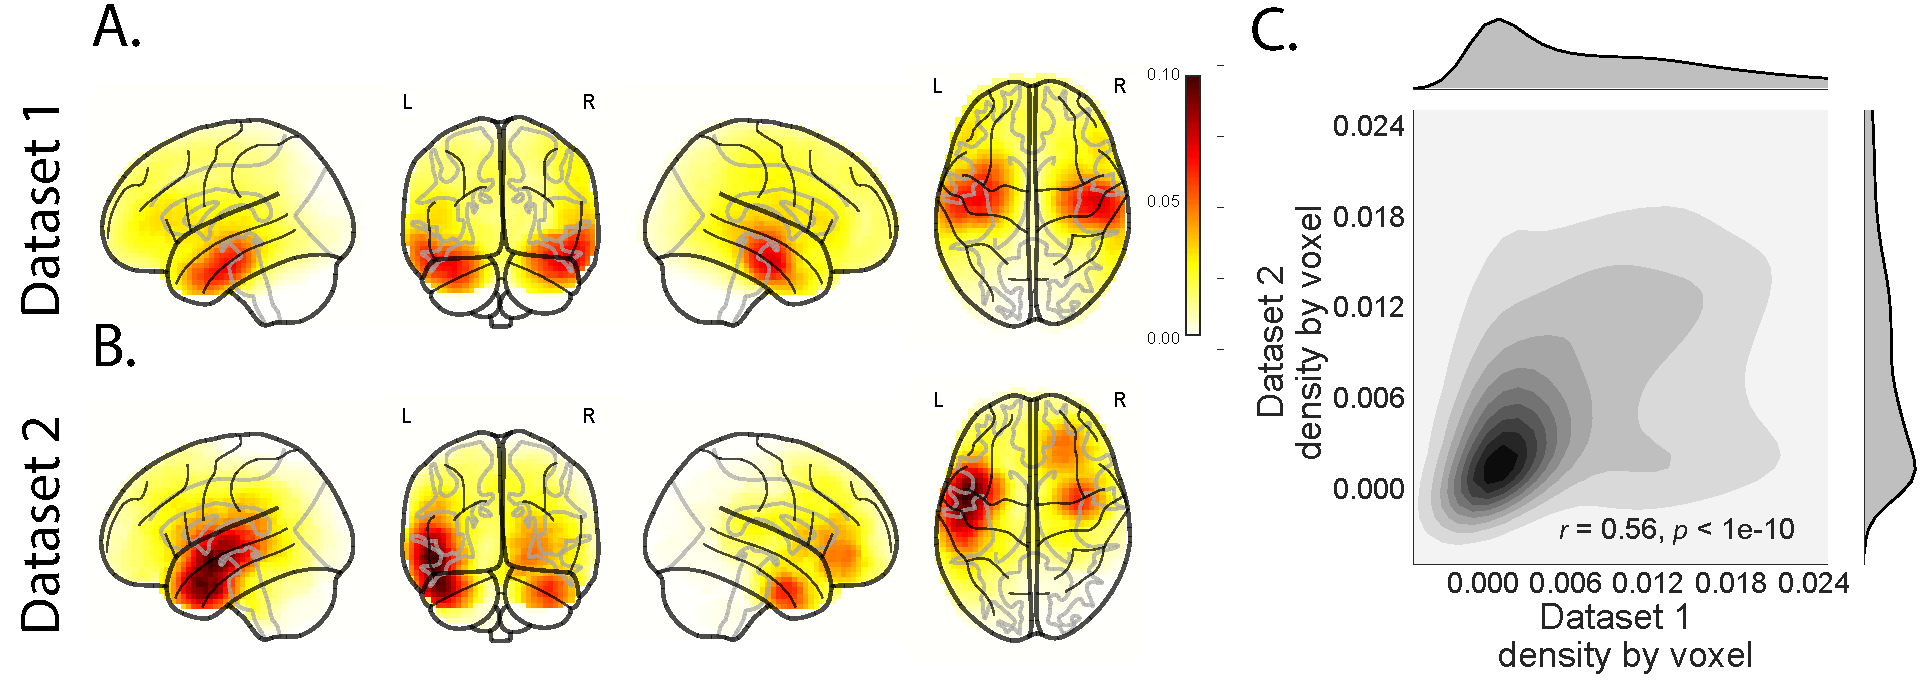
\includegraphics[width=\textwidth]{figs/density}
  \caption{\textbf{Sampling density and reconstruction quality.}
    \textbf{A. \& B. } The glass brain maps show sampling density by voxel location for dataset 1 and dataset 2. \textbf{C.}
      Correlation of sampling density by voxel location for dataset 1 vs. dataset 2.}
  \label{fig:density}
\end{figure}

In addition to exploring how reconstruction quality varies with
location, we also wondered whether there might be effects of electrode
placements on reconstruction quality.  For example, are there
particular implantation locations that yield especially high
reconstruction accuracies at other locations throughout the brain? To gain insights into this questions, we computed the average reconstruction correlation for each patient, then computed the average patient reconstruction correlation for any patients who had electrodes within a 20 MNI unit diameter sphere centered on each voxel location. The resulting maps highlight the locations of implanted electrodes from patients whose
reconstructions were especially accurate  (Fig.~\ref{fig:informap}A and B). We found that the most informative locations were consistent across datasets which lends support to the notion that different electrode location are more informative about activity across patients (Fig.~\ref{fig:informap}C); $r = 0.22, p < 10^{-10}$).  The locations in dark red might therefore be good candidate
implantation targets for neurosurgeons and neurologists who wish to
use Super EEG to reconstruct full-brain electrophysiological signals.
The above findings, that one can infer brain activity throughout a person's brain 
using recordings from a limited number of locations from that person's brain in conjunction with recordings from other people's brains, have deep
implications for the structure of brain data.  The first implication
is that the correlational structure of different people's brain data
is largely preserved across individuals. Despite recent evidence that different people have stable but reliably different resting state connectome~\cite{FinnEtal15}, our results suggest that the correlational structure of different people's brain data is preserved enough across individuals to provide meaningful information. 

\begin{figure}
  \centering
  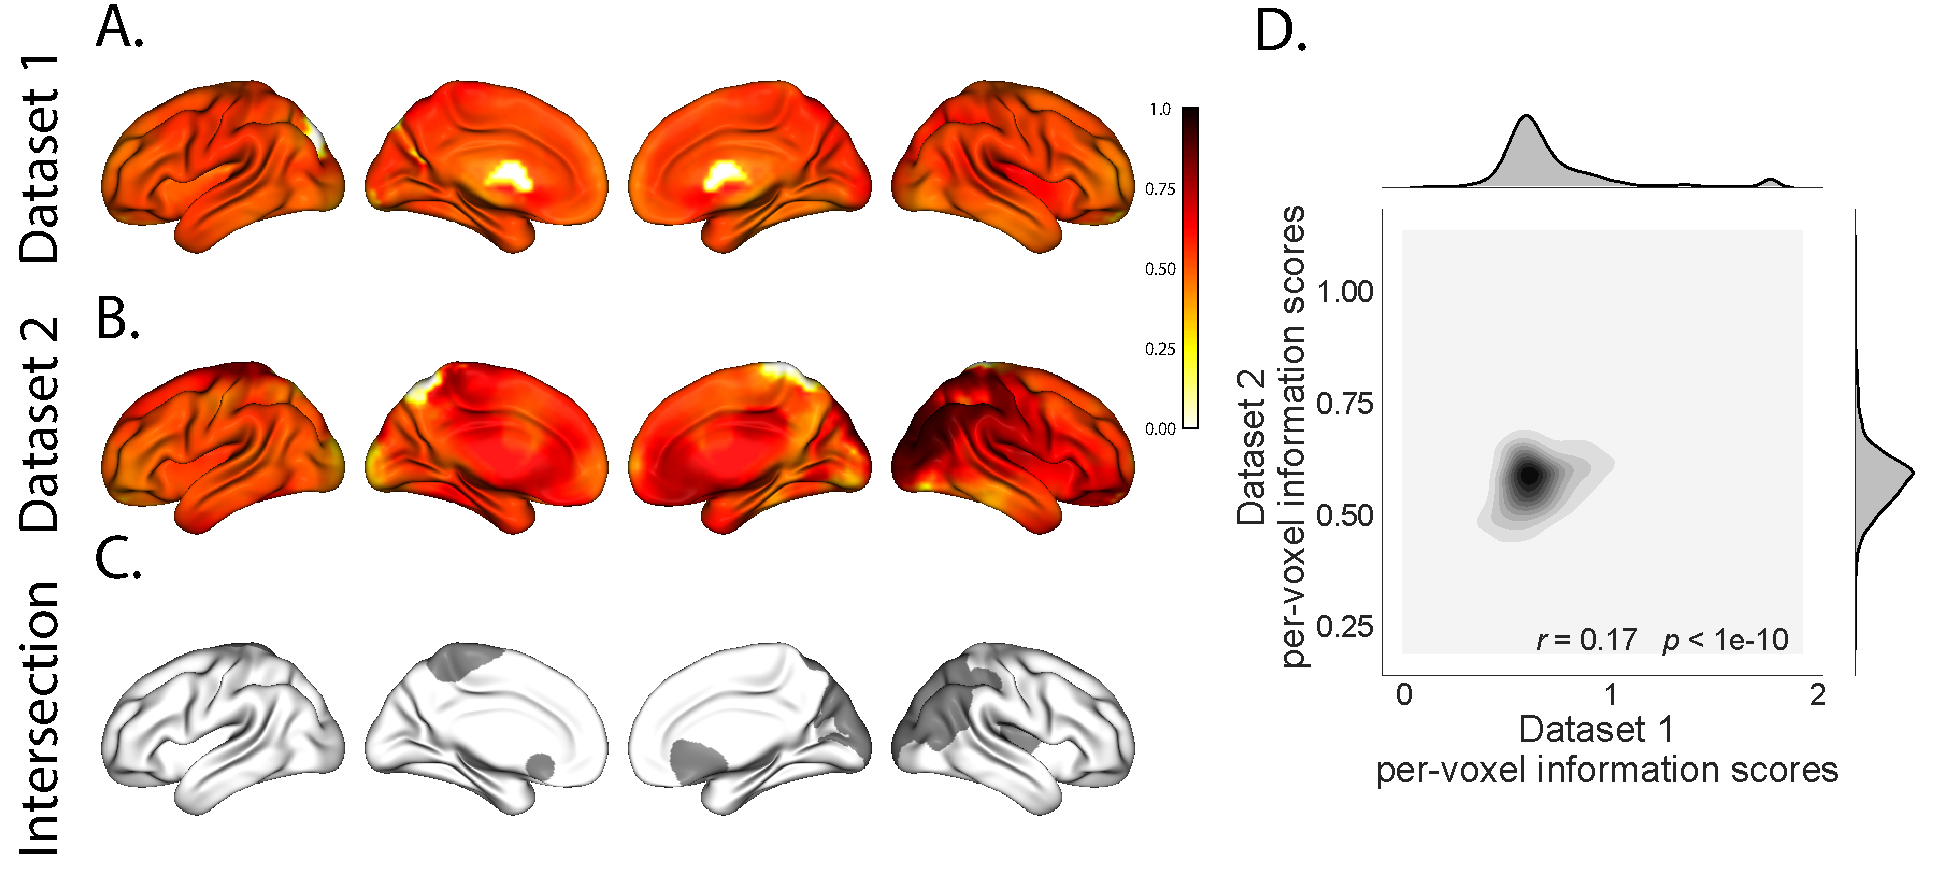
\includegraphics[width=\textwidth]{figs/informap}
  \caption{\textbf{Most informative electrode locations.} \textbf{A. \& B. } The glass
    brain maps displays the average reconstruction correlations (by patient, across
    all electrodes) for patients with electrodes within a 20 MNI unit diameter sphere centered on
    each location for dataset 1 and dataset 2. \textbf{C.} Correlation between z-transformed correlations by voxel for dataset 1 vs. dataset 2.}
  \label{fig:informap}
\end{figure}


\section*{Discussion}
%DISCUSSION POINTS
%recap main approach
Super EEG infers full-brain activity patterns by leveraging
correlations in those patterns of brain activity within and across people.  Although
the approach may, in principle, be used to infer brain activity
\textit{anywhere} in the brain, the inferences perform slightly better for
regions with dense electrode sampling across patients.  (Taken to the logical extreme, we could not hope to accurately recover activity patterns from brain areas where no recordings existed from any patient.)   As more data
are included in the inference procedure, this suggests that reconstruction accuracy should improve.

%why does it work?  redundancy of brain
A fundamental assumption of the Super EEG algorithm is that the data
covariance matrix is stable over time and across people.  This is a
useful simplification.  However, a growing body of evidence from the
fMRI community suggests that the data covariance matrix changes in
meaningful ways over time (for example, the data covariance matrix
changes from moment-to-moment during story listening, serving as a
unique ``fingerprint'' for each moment of the story; further, these
task-driven timepoint-specific covariance fingerprints appear to be
largely preserved across people~\cite{SimoEtal16, MannEtal17}).  These
findings indicate that the full-brain covariance matrix is not stable
over time.  Other recent work has shown that people's resting state
connectivity matrices may be used to uniquely identify individuals and
predict fluid intelligence scores~\cite{FinnEtal15}.  This indicates
that the full-brain covariance matrix is not stable across people.  If
the fundamental stability assumptions that Super EEG relies on are
violated, how can the Super EEG algorithm still accurately recover LFP
data?  It is important to recognize that the fact that variability
(over time or across people) is predictive (e.g.\ of cognitive states
during story listening or fluid intelligence scores) does not
necessarily mean that this variability is large in magnitude.  Rather,
we have long known that brain structure is tightly preserved across
individuals (and over time, at least on the timescale of typical
clinical and experimental recording sessions), and any functional
changes must occur within the framework of the underlying structural
anatomy.  Nevertheless, one could imagine future improvements to the
Super EEG approach that leverage resting state fMRI or structural data
[e.g. diffusion tensor imaging (DTI)] to estimate Bayesian priors over
the correlation matrices inferred, in the current framing, using only
ECoG data.  Further, relaxing the assumption that the covariance
matrix is stable (over time and/or across people), and/or
incorporating more detailed brain conductance models (e.g.\ informed
by structural MRI scans) may improve the predictive performance of the
approach.



%This technique relies on recordings from many patients performing the
%same basic cognitive task.  To what extent do these findings
%generalize across studies?  For example, could one combine recordings
%from several studies to improve our ability to reconstruct neural
%activity?
One potential limitation of the Super EEG approach is that the above
assumption of covariance stability across people may be violated even
more if different patients are performing different cognitive tasks.
To understand of the extent to which the current findings generalize across
cognitive tasks, we replicated our initial findings using a dataset in which patients participated in two tasks, and limited the training data to either within task, across task, or using both tasks. Since we found the most accurate reconstructions using task-specific data, this would suggest building up new databases for estimating each task-specific covariance
matrix.  Or, using a more sophisticated approach, one could create a
hierarchical model whereby each task-specific covariance matrix was
modeled as a perturbation of a ``global'' task-unspecific covariance
matrix (which could in turn be informed by fMRI or DTI data).
% Alternatively, if the covariance matrix is stable across tasks, this would
% suggest that recordings from multiple studies could be combined to
% improve the overall reconstruction accuracy.

A second potential limitation of the Super EEG approach is that it
does not provide a natural means of estimating the precise timing of
single-neuron action potentials.  Prior work has shown that gamma band
and broadband activity in the LFP may be used to estimate the firing
rates of neurons that underly the population contributing to the
LFP~\cite{MannEtal09}.  Because Super EEG reconstructs LFPs throughout
the brain, one could in principle use gamma or broadband power in the
reconstructed signals to estimate the corresponding firing rates
(though not the timings of individual action potentials).

Beyond providing a means of estimating ongoing activity throughout the
brain using already implanted electrodes, our work also has
implications for where to place the electrodes in the first place.
Electrodes are typically implanted to maximize coverage of suspected
epileptogenic tissue.  However, our findings suggest that this approach
could be further optimized.  Specifically, one could leverage not only
the non-invasive recordings taken during an initial monitoring period
(as is currently done), but also recordings collected from other
patients.  We could then ask: given everything we know about the other
patients and from the scalp recordings of this new patient, where
should we place a fixed number of electrodes to maximize our ability
to map seizure foci?  As shown in Figure~\ref{fig:informap}, recordings
from different locations are differently informative in terms of
reconstructing the spatiotemporal patterns throughout the brain.
This property might be leveraged in decisions about where to
surgically implant electrodes in future patients.


\section*{Concluding remarks}
Over the past several decades, neuroscientists have begun to leverage
the strikingly profound mathematical structure underlying the brain's
complexity to infer how our brains carry out computations to support
our thoughts, actions, and physiological processes.  Whereas
traditional beamforming techniques rely on geometric
source-localization of signals measured at the scalp, here we propose
an alternative approach that leverages the rich correlational
structure of a large dataset of human intracranial recordings.  In
doing so, we are one step closer to observing, and perhaps
someday understanding, the full spatiotemporal structure of human
neural activity.

\section*{Code availability}
We have released an open-source SuperEEG Python toolbox.  All of the code used in this manuscript is on GitHub, and the code may be shared using a GitHub account accessible to the reviewers upon request.

\section*{Data availability}
The dataset analyzed in this study was generously shared by Michael J. Kahana.  A portion of the dataset may be downloaded \href{http://memory.psych.upenn.edu/Request_EEG_access?paper=SedeEtal03}{\underline{here}}.
\section*{Acknowledgements}
We are grateful for useful discussions with Luke J. Chang and Matthijs van der Meer.  We are also grateful to Michael J. Kahana for generously sharing
the ECoG dataset we analyzed in our paper, which was collected under
NIMH grant MH55687 to MJK.  Our work was also supported in part by NSF EPSCoR Award Number 1632738.  The content is solely the responsibility of the authors and does not necessarily represent the official views of our supporting organizations.
\section*{Author Contributions}
J.R.M conceived and initiated the project. L.L.W.O. and A.C.H. performed the analyses. J.R.M. and L.L.W.O. wrote the manuscript.

\section*{Author Information}
Reprints and permissions information is available at www.nature.com/reprints.  The authors declare no competing financial interests.  Readers are welcome to comment on the online version of the paper.  Publisher's note: Springer Nature remains neutral with regard to jurisdictional claims in published maps and institutional affiliations.  Correspondence and requests for materials should be addressed to J.R.M.  (jeremy.r.manning@dartmouth.edu).

\bibliography{CDL-bibliography/memlab.bib}
\bibliographystyle{Science}

\clearpage

\end{document}




















